\usetikzlibrary{trees}
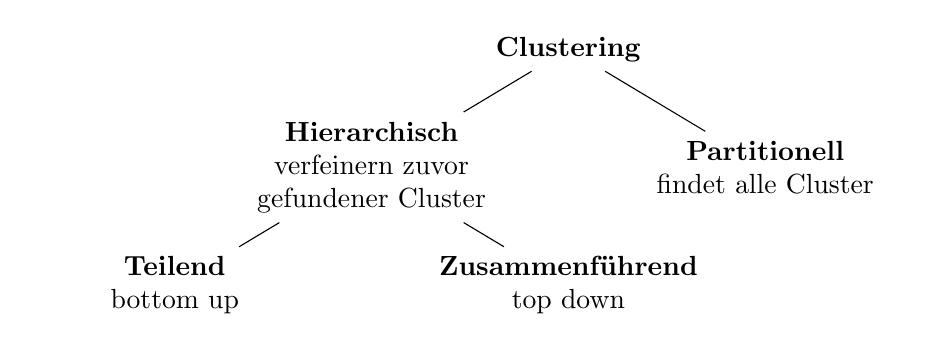
\begin{tikzpicture}[
	text width=3.5cm, align=flush center,
	level 1/.style={level distance=1.5cm, sibling distance=5cm},
	level 2/.style={}
]
	\node {\textbf{Clustering}}  % root {
		child { node {\textbf{Hierarchisch}\\verfeinern zuvor gefundener Cluster}
			child {node {\textbf{Teilend}\\ bottom up}}
			child {node {\textbf{Zusammenführend}\\ top down}}
		}
		child { node {\textbf{Partitionell} \\ findet alle Cluster} }
	;
\end{tikzpicture}
